\begin{definition}
    Будем говорить, что точка $x_0$ функции $f: \R \to \R$ является регулярной, если в ней $\exists f(x_0 \pm 0)$ и $\exists f'_\pm(x_0)$.
\end{definition}
\begin{corollary}[Из признака Дини]
    Пусть дана $2\pi$-периодическая функция $f \in L_1([-\pi, \pi])$. Тогда если $x_0$~---~регулярная точка функции $f$, то ряд Фурье $f$ сходится в ней к $\frac{f(x_0 + 0) + f(x_0 - 0)}{2}$.
\end{corollary}
\begin{proof}
    Для доказательства в силу признака Дини достаточно проверить, что $\exists \delta > 0$ такое, что \[
                                                                                                          \int_0^\delta \bigg|f(x_0 + u) - f(x_0 + 0) + f(x_0 - u) - f(x_0 - 0)\bigg|\dfrac{du}{u} < +\infty.
    \]
    Поскольку \[
                  \dfrac{f(x_0 + u) - f(x_0 + 0)}{u} \rightarrow f'_+(x_0), u \rightarrow +0 \quad  \dfrac{f(x_0 - u) - f(x_0 - 0)}{u} \rightarrow f'_-(x_0), u \rightarrow +0.
    \]
    То есть существует $\delta > 0$ такое, что
    \[
        \biggr|\dfrac{f(x_0 + u) - f(x_0 + 0)}{u}\biggr| \in \biggr[\dfrac{|f'_+(x_0)|}{2}, 2|f'_+(x_0)|\biggr] \quad \biggr|\dfrac{f(x_0 - u) - f(x_0 - 0)}{u}\biggr| \in \biggr[\dfrac{|f'_-(x_0)|}{2}, 2|f'_-(x_0)|\biggr] \forall u \in (0, \delta).
    \]
    А значит выполнено условие Дини и ряд сходится к полусумме односторонних пределов.
\end{proof}

\begin{fact}
    Для любой непрерывной $2\pi$ периодической функции ее ряд Фурье сходится к ней почти всюду (следует из теоремы Карлесона)
\end{fact}



\begin{example}[Шварц]
    Существует непрерывная $2\pi$-периодическая функция такая, что её ряд Фурье расходится в нуле. \\
    Определим функцию $f$ как \[
                                  f(t) =
                                  \begin{cases}
                                      0, & t = 0 \\
                                      \dfrac{1}{\sqrt{k}}\sin n_kt, & t \in [t_k, t_{k - 1}], k = 2, \ldots
                                  \end{cases}
    \]
    где $n_k = 2^{k!}$, $t_1 = \pi$ и $t_k = \frac{2\pi}{n_k}, k > 1$.
    \begin{center}
        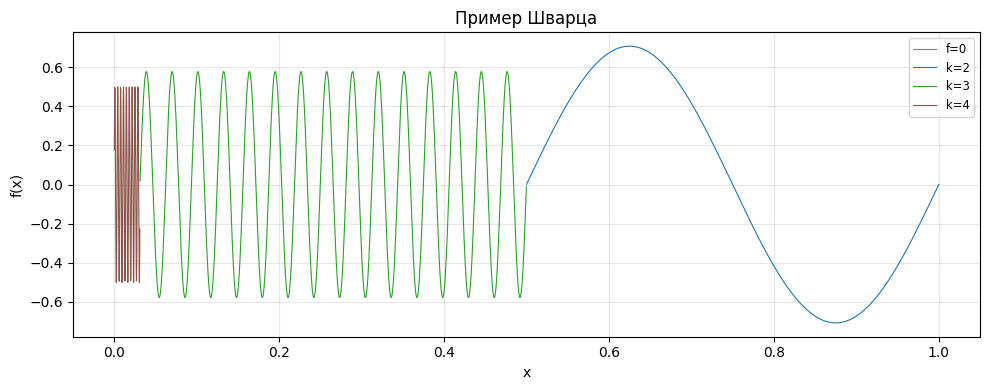
\includegraphics[width=1\linewidth]{Pictures/Shwartz.png}
    \end{center}

    Определим $J_n[f]$ как \[
                               J_n[f](0) = \int_0^\pi \dfrac{\sin nt}{t}f(t)dt.
    \]
    Исследуем поведение $J_n[f]$ на гармониках $n_k$:
    \[
        J_{n_k}[f](0) = \int_0^\pi \dfrac{\sin n_kt}{t}f(t)dt = \int_0^{t_k}\dfrac{\sin n_kt }{t}f(t)dt + \int_{t_k}^{t_{k - 1}}\dfrac{\sin^2 n_kt}{t \sqrt{k}}dt + \int_{t_{k - 1}}^\pi \dfrac{\sin n_kt}{t}f(t)dt = F_k + J_k + H_k.
    \]
    Рассмотрим для начала поведение интеграла $J_k$:
    \[
        \dfrac{1}{\sqrt{k}}\int_{2\pi}^{A_k}\sin^2 \tau \dfrac{d\tau}{\tau} = \dfrac{1}{\sqrt{k}}\int_{2\pi}^{A_k}\dfrac{1 - \cos 2\tau}{2\tau}d\tau.
    \]
    где $A_k = 2\pi \frac{n_k}{n_{k - 1}}$. Заметим, что \[
                                                             \int_{2\pi}^{+\infty}\dfrac{\cos 2\tau}{\tau}d\tau.
    \]
    сходится по признаку Дирихле, а значит \[
                                               \exists C > 0 \ \forall k \in \N \hookrightarrow \biggr|\int_{2\pi}^{A_k} \dfrac{\cos 2\tau}{2\tau}d\tau\biggr| < C.
    \]
    С другой стороны, \[
                          \int_{2\pi}^{A_k} \dfrac{d\tau}{2\tau} = \ln \dfrac{A_k}{2\pi} = \dfrac{1}{2}(k! - (k - 1)!)\ln 2 \geq \dfrac{k! \ln 2}{3}.
    \]
    А значит \[
                 J_k \geq \dfrac{\ln 2}{3\sqrt{k}}k! + O(1).
    \]
    Оценим $H_k$: \[
                      |H_k| \leq \ln \dfrac{\pi}{t_{k - 1}} = \ln \dfrac{n_{k - 1}}{2} \leq (k - 1)!\ln 2.
    \]
    И последний интеграл: \[
                              |F_k| \leq \int_0^{t_k} \biggr|\dfrac{\sin n_kt}{t}f(t)\biggr|dt \leq \int_0^{t_{k}}\dfrac{|\sin n_kt|}{t}|f(t)|dt \leq \int_0^{t_k}|n_kf(t)|dt \leq \dfrac{n_k t_k}{\sqrt{k}} = \dfrac{2\pi}{\sqrt{k}} \rightarrow 0, k \rightarrow +\infty.
    \]
    Таким образом, получается: \[
                                   J_{n_k}[f](0) \geq \dfrac{\ln 2}{3\sqrt{k}}k! + O(1) - (k - 1)!\ln 2 - \dfrac{2\pi }{\sqrt{k}} \geq (k - 1)!\ln 2(\dfrac{\sqrt{k}}{3} - 1) + O(1) \rightarrow +\infty, k \rightarrow +\infty.
    \]
    А значит $S_{n_k}[f](0) \rightarrow +\infty, k \rightarrow +\infty$ и ряд Фурье функции $f$ расходится в нуле.
\end{example}
% Пересмотреть, дополнить <<неформальность>>.
\subsection{Суммы Фейера}
Неформальная идея. При рассмотрении обычных числовых рядов, возникала ситуация $1 + (-1) + 1 + (-1) + 1  + \dots$ это расходящийся ряд, так как нет предела частичных сумм. Но вот если мы рассмотрим $\Sigma_n = \frac{S_1 +\dots +S_n}{n} \to \frac{1}{2}$. С рядами Фурье часто происходит также. Поэтому мы рассматриваем ряды Фейера, как аналог $\Sigma_n$.


\begin{definition}
    Пусть дана $2\pi$-периодическая $f \in L_1([-\pi, \pi])$. Суммой Фейера для $f$ будем называть \[
                                                                                                       \sigma_n[f] = \dfrac{1}{n}\sum\limits_{i = 0}^{n - 1} S_i[f].
    \]
\end{definition}
Распишем подробнее сумму Фейера через выражение для ядер Дирихле:
\[\sigma_n[f](x) = \dfrac{1}{2\pi n}\int_{-\pi}^{\pi} \dfrac{f(x  - u)}{\sin u/2}\sum\limits_{k = 0}^{n - 1} \sin (k + 1/2)u du.\]
В тоже время, \[
                  \dfrac{1}{\sin u/2}(\sin u/2 + \ldots + \sin (n - 1/2)u)\sin u/2 = \dfrac{1}{2\sin u/2}(1 -\cos nu).
\]
\begin{definition}
    Ядром Фейера будем называть \[
                                    \Phi_n = \dfrac{1}{n}\sum\limits_{k = 0}^{n - 1}D_k = \dfrac{\sin^2 nu/2}{2\pi n \sin^2 u/2}.
    \]
\end{definition}
Тогда сумма Фейера для $f$ может быть записана как свёртка ядра Фейера и функции $f$: \[
                                                                                          \sigma_n[f](x) = \Phi_n * f = \int_{-\pi}^{\pi} \Phi_n(x- u)f(u)du.
\]
Ядро Фейера можно также записать в виде \[
                                            \Phi_n(u) = \dfrac{1}{n}\sum\limits_{k = 0}^{n - 1}D_k(u) = \dfrac{1}{2\pi n}\sum\limits_{k = 0}^{n - 1}\sum\limits_{|j| < k} e^{iku} = \dfrac{1}{2\pi}\sum\limits_{|k| < n} \biggr(1 - \dfrac{|k|}{n}\biggr)e^{iku}
\]
% Дописать технические подробности.
\begin{proposition}
    Нетрудно заметить некоторые свойства ядра Фейера:
    \begin{itemize}
        \item $\forall n \in \N \hookrightarrow\Phi_n \geq 0$.
        \item $\Phi_n$~---~$2\pi$-периодичная функция.
        \item Поскольку $\int_{-\pi}^{\pi}D_n(u)du = 1$, то \[
                                                                \int_{-\pi}^{\pi} \Phi_n(u)du = \dfrac{1}{n}\sum\limits_{k = 0}^{n - 1}\int_{-\pi}^{\pi} D_n(u)du = 1.
        \]
        \item Для ядра Фейера справедливо т.н. <<фокусирующее свойство>>: \\ при всяком $\delta > 0$ и $\delta < |u| < \pi$ верно
        \[
            \Phi_n(u) = \dfrac{1}{2\pi n}\biggr(\dfrac{\sin nu/2}{\sin u/2}\biggr)^2 \leq \dfrac{1}{2\pi n \sin^2 \delta /2} \leq \dfrac{\pi}{2n\delta^2} \rightarrow 0, n \rightarrow +\infty.
        \]
        Таким образом, \[
                           \forall \delta > 0 \hookrightarrow \sup\limits_{\delta < |u| < \pi} \Phi_n(u) \rightarrow 0, n \rightarrow +\infty.
        \]
    \end{itemize}
\end{proposition}
\begin{definition}
    Будем говорить, что для $\alpha \in (0, 1)$ функция лежит в $H^\alpha(\R)$ (т.е. удовлетворяет условию Гёльдера с показателем $\alpha$) если \[
                                                                                                                                                     \exists C > 0 \forall x', x'' \in \R \hookrightarrow |f(x') - f(x'')| \leq C|x' - x''|^\alpha.
    \]
    При $\alpha = 1$ это условие Липшица.
\end{definition}
\begin{theorem}
    Пусть дана $2\pi$-периодическая $f \in H^\alpha(\R), \alpha \in (0, 1)$. Тогда ряд Фурье $f$ сходится к ней равномерно на $\R$. Более того, \[
                                                                                                                                                    \biggr|S_n[f](x) - f(x)\biggr| \leq C \cdot \dfrac{\ln n}{n^\alpha} \quad \forall n \in \N, \forall x \in \R.
    \]
\end{theorem}
\begin{proof}
    Для начала рассмотрим отклонения от суммы Фейера и, вставив <<умную $1$>>, с помощью ее интегрального свойства получим:
    \[
        \sigma_n[f](x) - f(x) = \int_{-\pi}^\pi f(x - t)\Phi_n(t)dt - \int_{-\pi}^{\pi}\Phi_n(t)f(x)dt = \int_{-\pi}^{\pi} (f(x - t) - f(x))\Phi_n(t)dt.
    \]
    То есть \[
                |\sigma_n[f](x) - f(x)| \leq \int_{-\pi}^{\pi}|f(x - t) - f(x)|\Phi_n(t)dt \leq \dfrac{C}{2\pi n} \int_{0}^{\pi} t^\alpha \cdot \dfrac{\sin^2 (nt/2)}{\sin^2 t/2}dt \leq (*)
    \]
    Но поскольку $\sin t/2 \geq \dfrac{2}{\pi} \cdot \dfrac{t}{2} = \dfrac{t}{\pi}$, то \[
                                                                                            (*) \leq \dfrac{C\pi}{2n} \int_0^{\pi} t^{\alpha - 2}\sin^2(nt/2)dt = (*)
    \]
    Теперь сделаем замену $nt/2 = u$ и получим \[
                                                   (*) = \dfrac{C \pi}{2 n} \int_0^{\pi n/2} \biggr(\dfrac{2u}{n}\biggr)^{\alpha - 2}\cdot\sin^2 u\cdot \dfrac{2}{n}du \leq \dfrac{2^{\alpha - 2}C \pi}{n^\alpha}\int_0^{\pi n / 2} \dfrac{\sin^2 u}{u^{2 - \alpha}}du.
    \]
    Но $\displaystyle \int_0^{+\infty}\frac{\sin^2 u}{u^{2 - \alpha}}du$ сходится в несобственном смысле, а значит $\exists \widetilde{C} > 0$ такая, что \[
                                                                                                                                                              \biggr|\int_0^{\pi n / 2}\dfrac{\sin^2 u}{u^{2 - \alpha}}du\biggr| \leq \widetilde{C}.
    \]
    И отклонение суммы Фейера от функции оценивается как \[
                                                             |\sigma_n[f](x) - f(x)| \leq \dfrac{M}{n^\alpha}.
    \]
    Пусть $\phi_n = f -\sigma_n[f]$. Cумма Фейера -- это тригонометрический полином $n$-ой степени, поэтому $S_n[\sigma_n[f]] = \sigma_n[f]$, а значит
    \[
        \big|S_n[\phi_n](x) - \phi_n(x)\big| = \big|S_n[f](x) - \sigma_n(x) - f(x) + \sigma_n(x) \big| = \big|S_n[f](x) - f(x)\big|.
    \]

    Тогда
    \[                                                                           \big|S_n[f](x) - f(x)\big| \leq \big|S_n[\phi_n](x)\big| + \big|\phi_n(x)\big| = (*)
    \]
    Оценка для $\phi_n$ уже есть выше.
    Для оператора частичной суммы некоторой $2\pi$-периодической функции $g$ мы можем дать следующую оценку:
    \begin{multline*}
        S_n[g](x) \leq \int_{-\pi}^{\pi}|g(x - t)|\biggr|\dfrac{\sin (n + 1/2)t}{\sin t/2}\biggr|dt \leq \\ \leq 2\sup\limits_{[-\pi, \pi]}|g| \cdot \int_{0}^\pi \biggr|\dfrac{\sin (n + 1/2)t}{\sin t/2}\biggr| dt \leq \\ \leq C_1 \sup |g| \int_0^{\pi (n + 1/2)} \dfrac{|\sin v|}{v}dv \leq \widetilde{C}\sup|g| \ln n.
    \end{multline*}
    Таким образом \[
                      (*) \leq \widehat{C}\dfrac{M\ln n}{n^\alpha}.
    \]
    Что доказывает равномерную сходимость и показывает требуемую оценку на отклонение частичной суммы.
\end{proof}